\chapter{Implementation}
\label{chapter:implementation}

To create an Application which can integrate into the daily lifes of someone, we will use the Flutter Technology Stack to create Software which can be accessed from many different platforms. For Developement, we focused on the usage of the Application on an Android Mobile Phone, however if we would like to expand our Application onto different plattforms, it would not require a lot of additional work.

Because we already defined the different Inputs which the user has access to, as described in Chaopter \ref{chapter:introducion}, we could immediately start with Implementation.

\begin{figure}[!ht]
	\centering
	\resizebox{0.5\textwidth}{!}{%
		\begin{circuitikz}
			\tikzstyle{every node}=[font=\Large]
			\draw [ rounded corners = 19.2] (3.25,5) rectangle (19.5,14.75);
			\draw  (3.75,5.5) -- (9.25,5.5) -- (9.75,8) -- (4.25,8) -- cycle;
			\node [font=\LARGE] at (6.75,6.75) {DetailsView};
			\draw  (12.75,5.5) -- (18.25,5.5) -- (18.75,8) -- (13.25,8) -- cycle;
			\node [font=\LARGE] at (15.75,6.75) {ResultsView};
			\draw [->, >=Stealth] (9.5,6.75) -- (13,6.75)node[pos=0.5, fill=white]{Gift Information};
			\draw  (13,14) rectangle  node {\Large OpenAI API Manager} (18.5,11.25);
			\draw [->, >=Stealth] (15,8) -- (15,11.25)node[pos=0.3, fill=white]{Gift Information};
			\draw [->, >=Stealth] (16.75,11.25) -- (16.75,8)node[pos=0.25, fill=white]{UI Gift Components};
			\node [font=\Large] at (6,14) {Flutter Android App};
			\draw  (15.75,19) ellipse (3.75cm and 1.25cm) node {\Large OpenAI API} ;
			\node [font=\Large] at (11.5,9.75) {};
			\draw [->, >=Stealth] (15,14) -- (15,17.75)node[pos=0.45,undefined, fill=white]{User Request};
			\draw [->, >=Stealth] (16.75,17.75) -- (16.75,14)node[pos=0.3,undefined, fill=white]{JSON Response};
		\end{circuitikz}
	}%

	\caption{Planned architecture of the App}
	\label{fig:architecture}
\end{figure}

Figure~\ref{fig:architecture} describes the planned architecture of the Flutter App. It has two main screens, which the User is guided throug:
\begin{enumerate}
	\item In the \texttt{DetailsView}, the User can specify different attributes about the Person they would like to gift something to (furthermore called the Recipient)

	\item As soon as the User submits the Information, all Gift Information is Passed to the \texttt{ResultsView}.

	\item The \texttt{ResultsView} passes the recieved Information to the API Manager, which converts it into a prompt, which is then sent to the OpenAI API.

	\item The OpenAI Assistant processes the Request and returns a Response in Form of a JSON Object. (For more details see Section~\ref{sec:backend})

	\item The API Manager recieves the JSON Object, extracts the relevant Information and sends it to the \texttt{ResultsView} in Form of prebuilt widgets, where they are displayed to the User.
\end{enumerate}

\section*{OpenAI API Manager}

The \texttt{OpenAI API Manager} is the backend logic which allows the Application to communicate with the OpenAI Assistant. It provides the functionality to convert User Input into a usable text prompt, as well as convert the recieved JSON into a nice Interface.

\begin{lstlisting}[language=Java]
    factory GiftResponse.fromJson(Map<String, dynamic> data) {
        GiftResponse gr = GiftResponse();
        for (Map<String, dynamic> idea in data['presents']) { // Extract "present" objects
          gr.ideas.add(Idea(idea["title"], idea['description'])); // Fill information into new Idea() Object
        }
        return gr; // Return a GiftResponse() Object containing Ideas()
    }

    
    List<Widget> cards(Set<Idea> ideas) {
        List<Widget> cards = List.empty(growable: true);
        for (Idea idea in ideas) { // For all Ideas in the List
            cards.add(Card( // Add a new widget (Flutter Card Widget in this Case)
            child: ListTile(
                title: Text(idea.title), // Title
                subtitle: Text(idea.description), // Description
                trailing: IconButton( // Shopping Bag Button
                    onPressed: () {
                        _launchUrl(
                            "https://www.galaxus.ch/de/search?searchSectors=0&q=${idea.title}");
                    },
                    icon: Icon(Icons.shopping_bag_outlined, color: Colors.green,))),
            ));
        }
        return cards;
    }
\end{lstlisting}

\section*{User Interface}

For the Design, we wanted a simple but clear User Interface. We used the  \href{https://m3.material.io/}{Material Design Guidelines} to ensure a consitent Design. At first, we created a simple UI which allows us to test the functionality of the app.

\begin{figure}

	\begin{subfigure}{0.5\textwidth}
		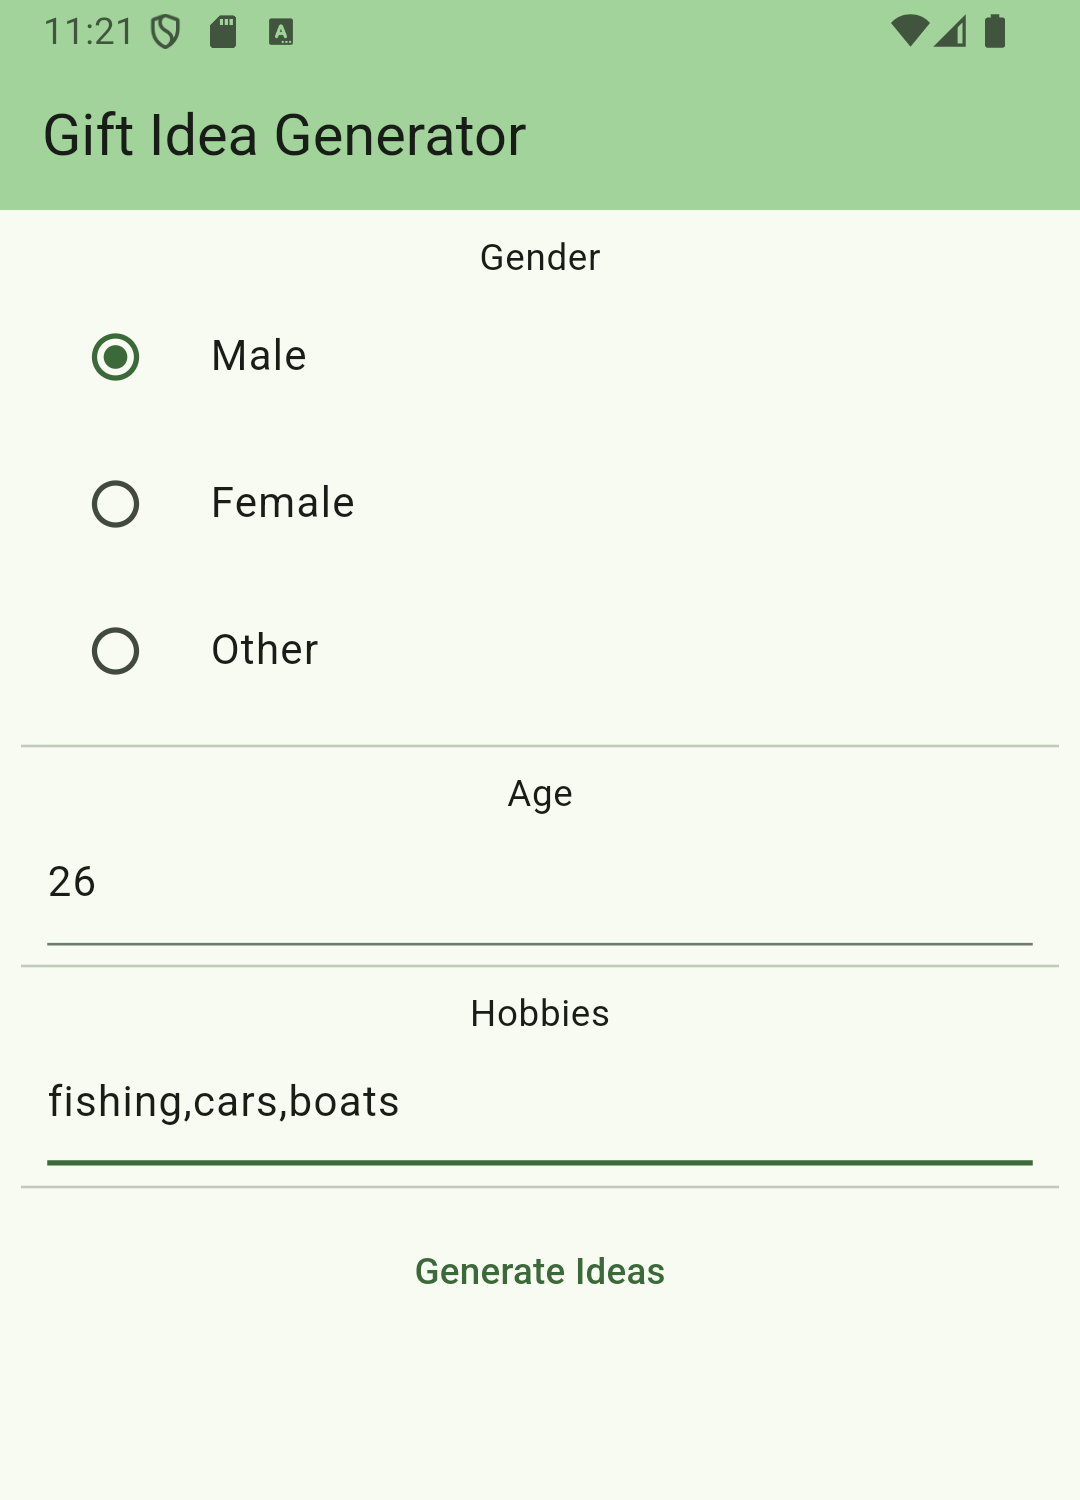
\includegraphics[width=0.9\linewidth]{figures/screenshots/old_details_view_cropped.png}
		\caption{\texttt{DetailsView}}
	\end{subfigure}
	\begin{subfigure}{0.5\textwidth}
		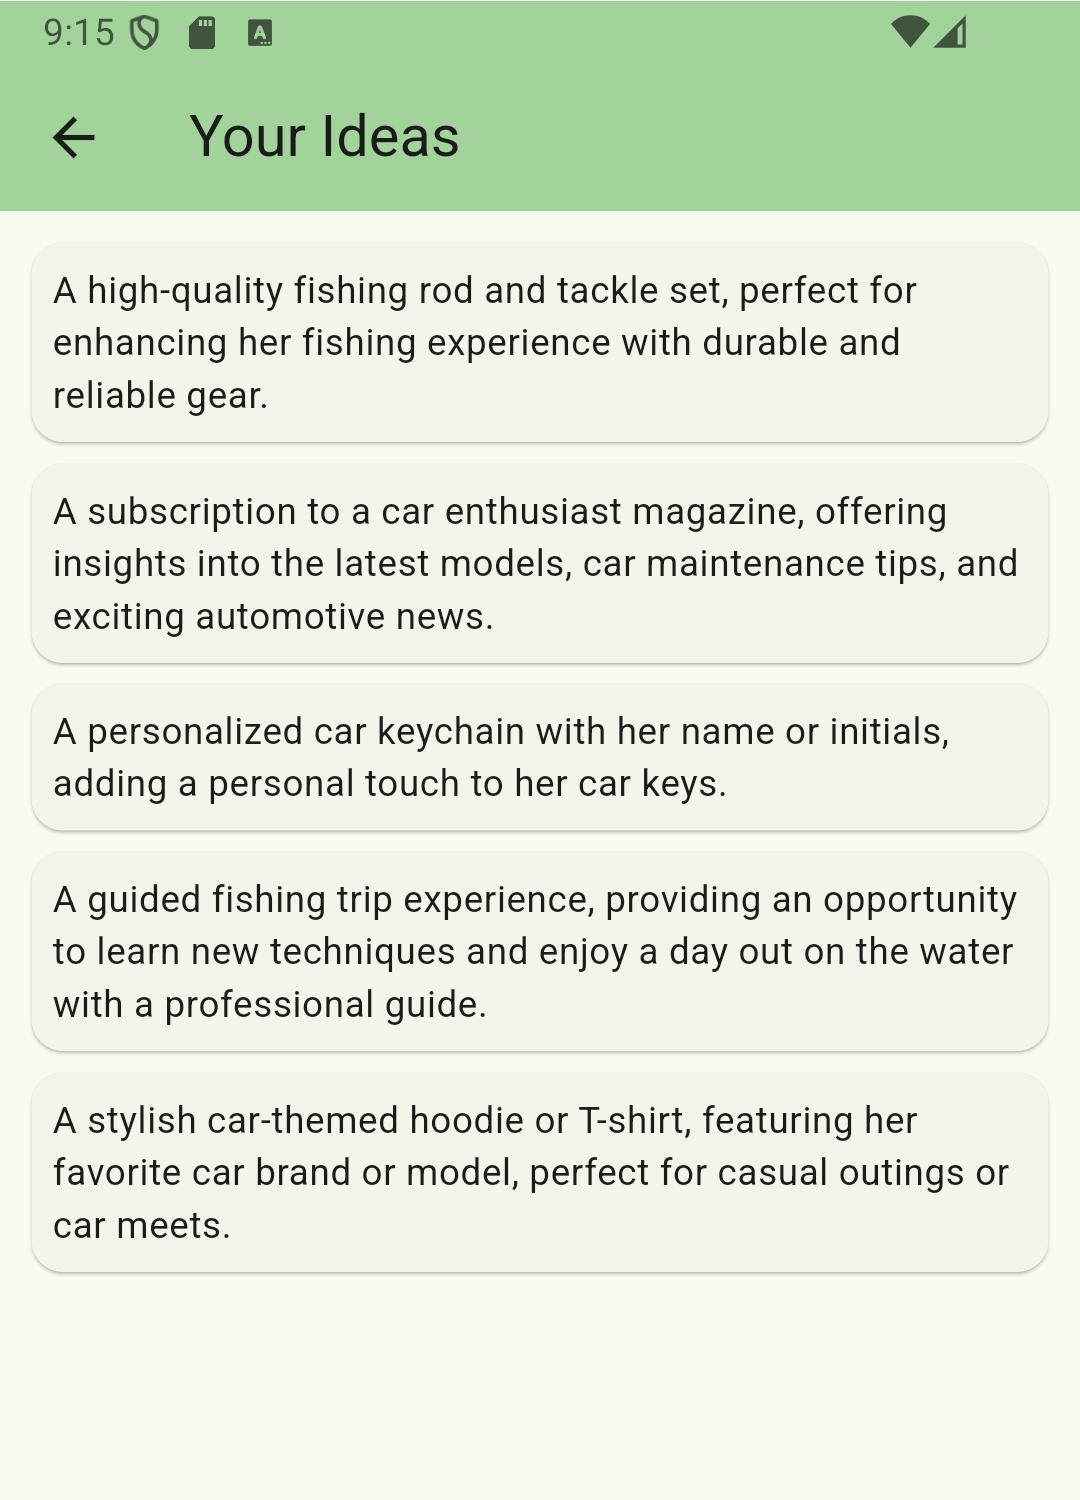
\includegraphics[width=0.9\linewidth]{figures/screenshots/old_results_view_cropped.png}
		\caption{\texttt{ResultsView}}
	\end{subfigure}
	\caption{Initial Version of the Application}
	\label{fig:initialVersion}
\end{figure}

After building the First version of the app as shown in Figure \ref{fig:initialVersion}, we proceeded to test the functionality of the API Manager, which provides the conversion from JSON Response to visually appealing Widgets.

Once the functionality has been confirmed, we focused on improving the UI. Although not our main focus of this project, we felt that a better UI can improve the overall impression of the Application significantly. We therefore implemented the following changes:

\begin{itemize}
	\item A small infobox which instructs potential first-time users.

	\item Improved display of input fields age and hobbies.

	\item The option to specify the Gender when selecting "Other"

	\item Title for each Idea to improve overview

	\item A button to instantly search for a gift on \url{galaxus.ch}
\end{itemize}

\begin{figure}

	\begin{subfigure}{0.5\textwidth}
		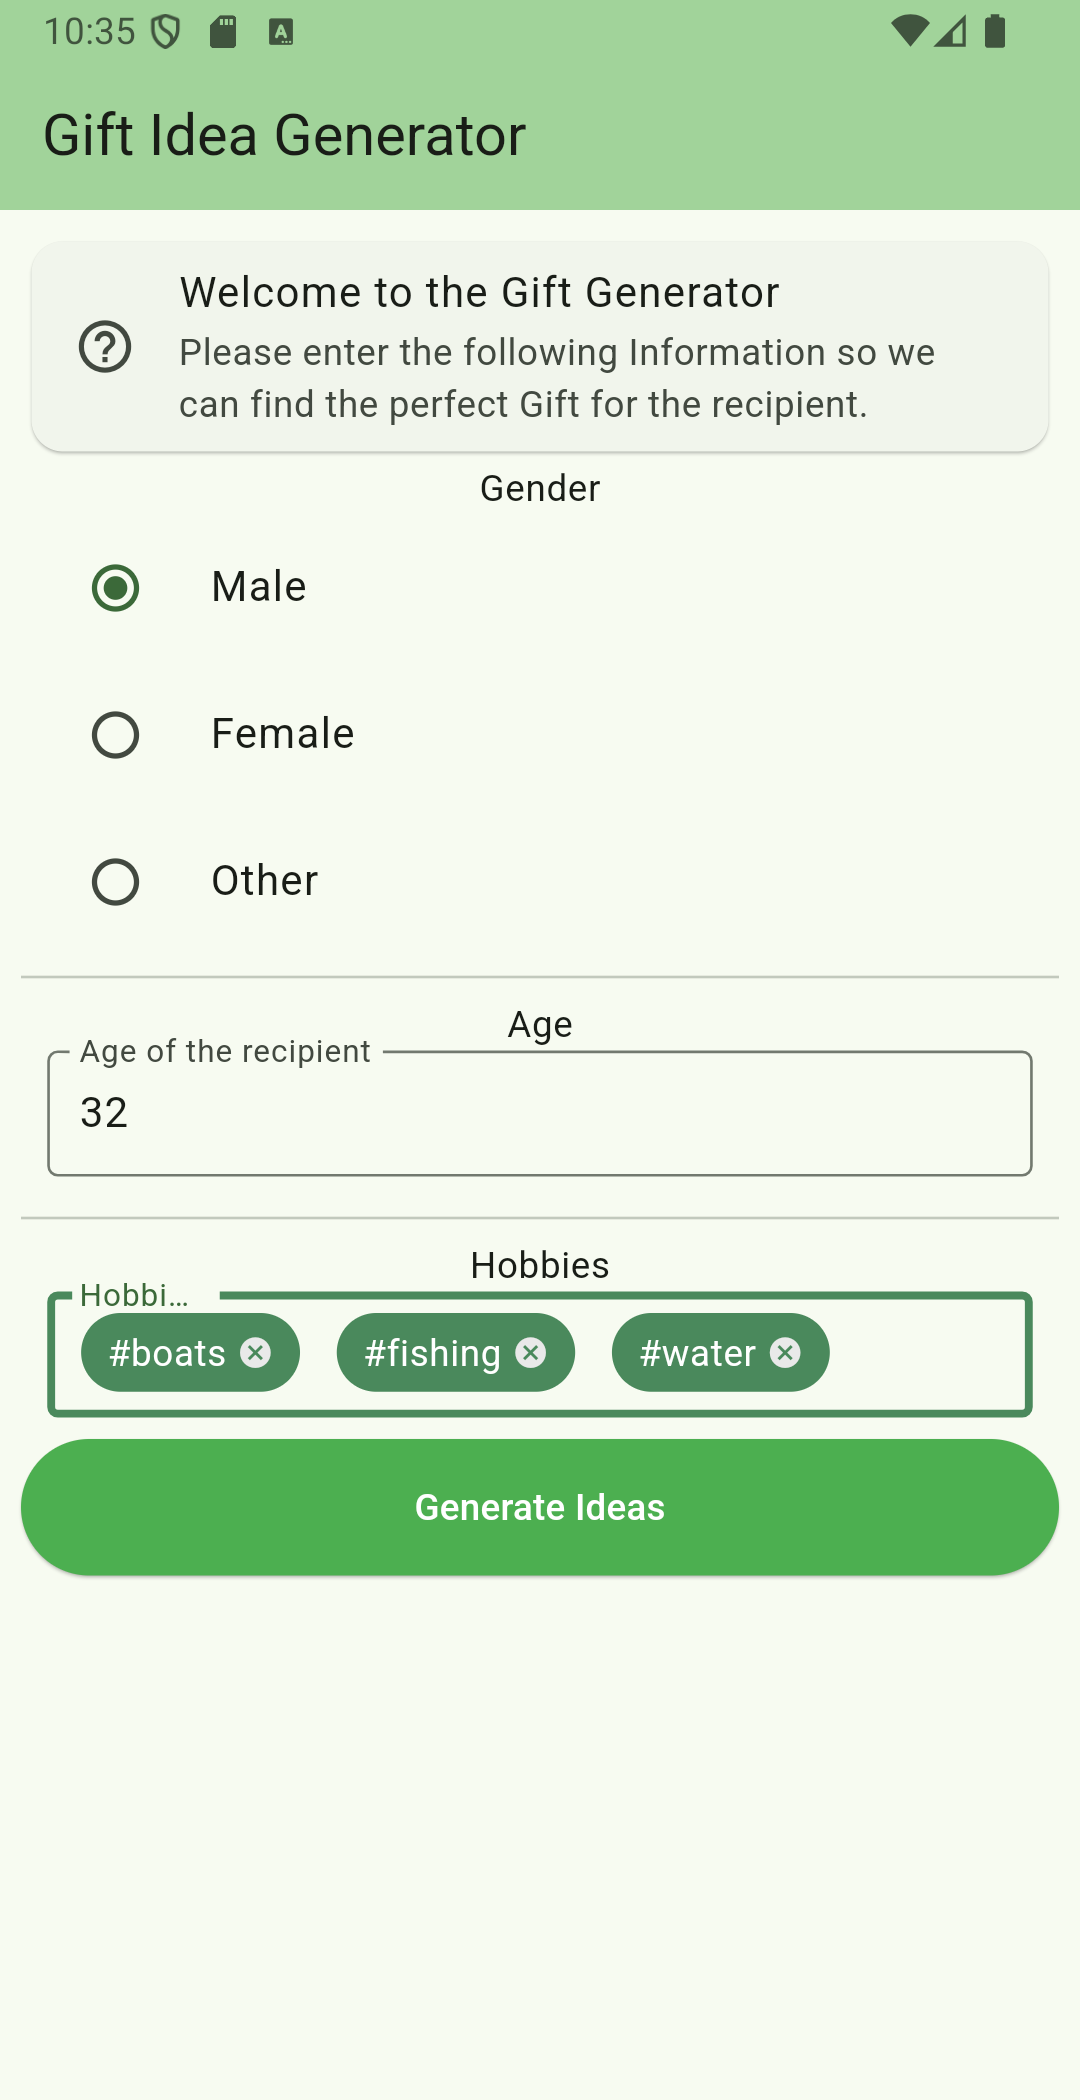
\includegraphics[width=0.9\linewidth]{figures/screenshots/new_details_view_cropped.png}
		\caption{\texttt{DetailsView}}
	\end{subfigure}
	\begin{subfigure}{0.5\textwidth}
		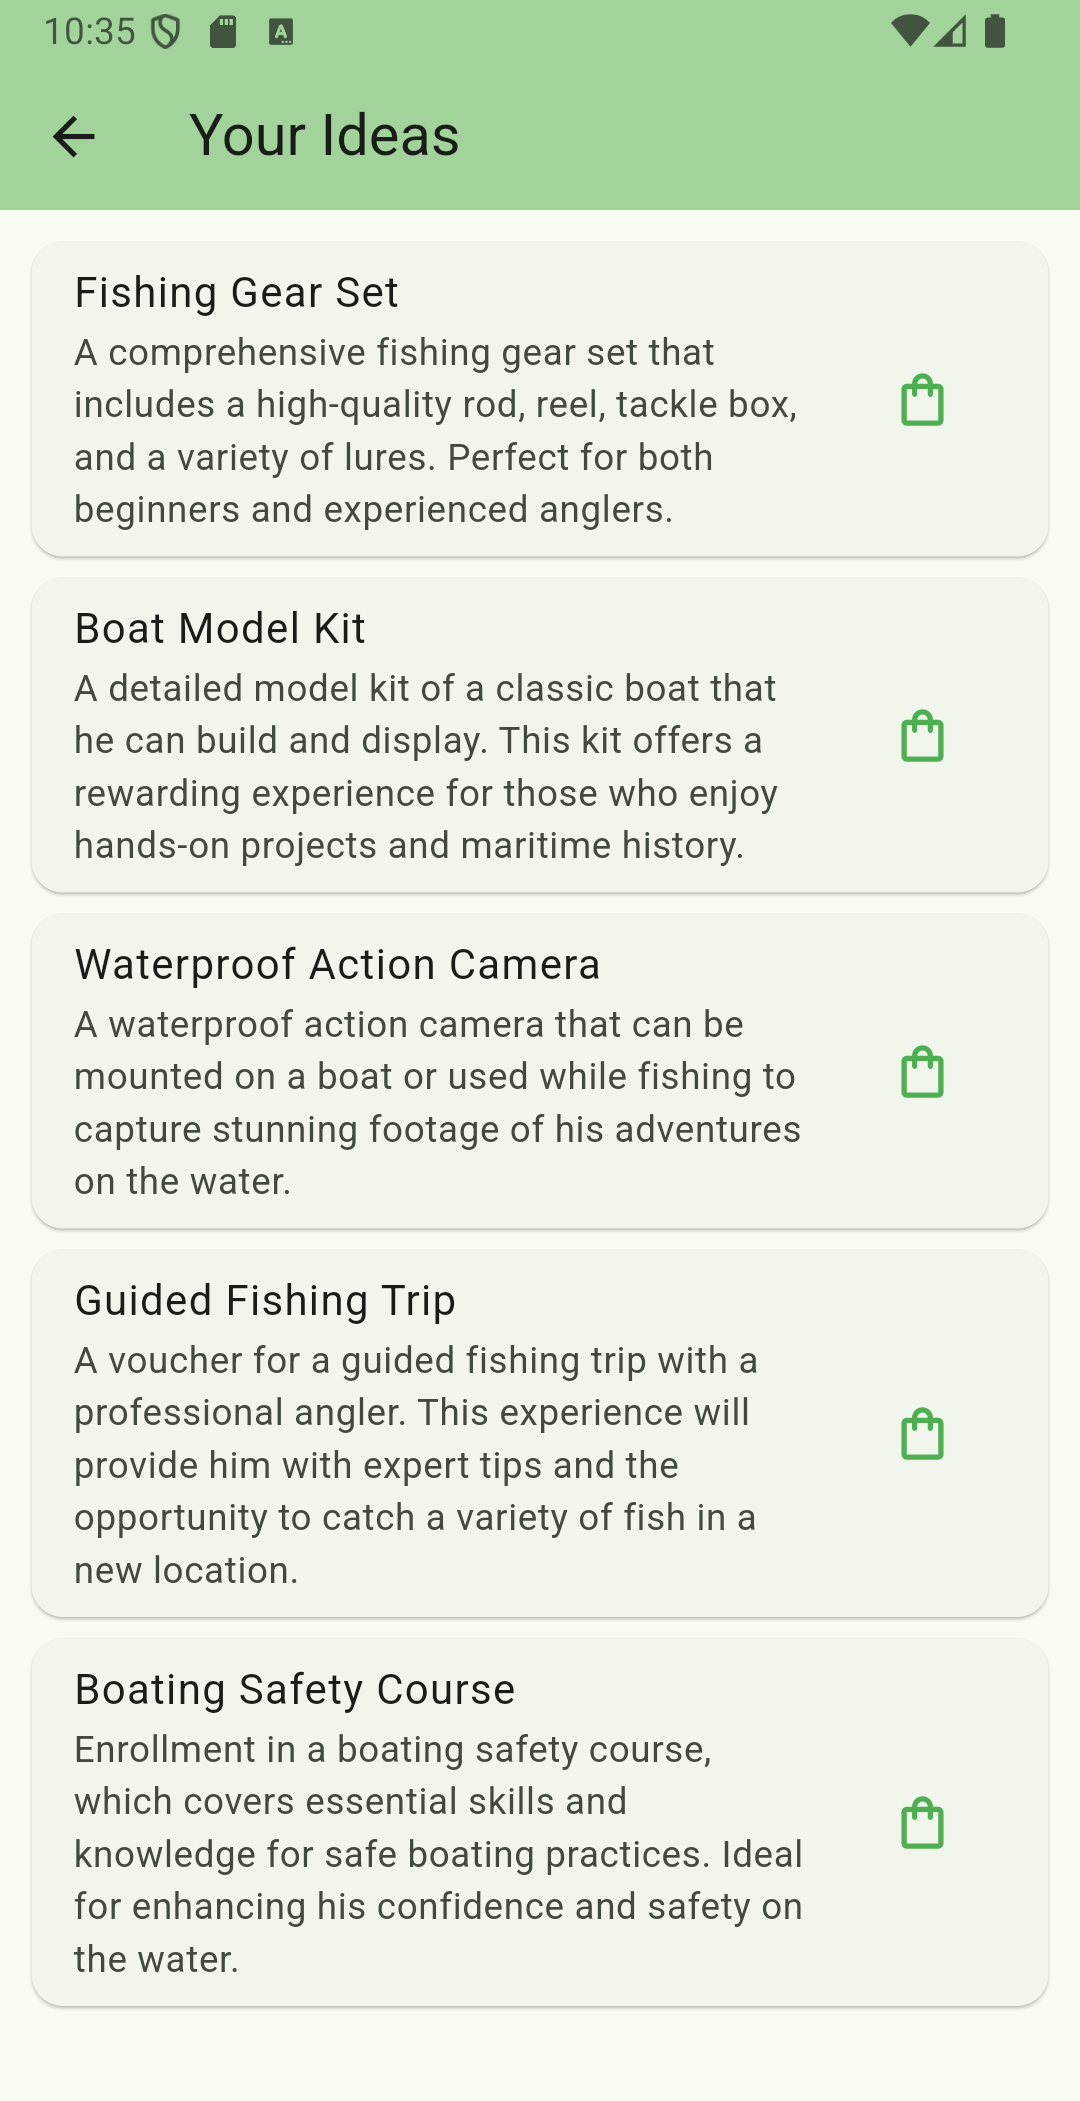
\includegraphics[width=0.9\linewidth]{figures/screenshots/new_results_view_cropped.png}
		\caption{\texttt{ResultsView}}
	\end{subfigure}
	\caption{Final Version of the Application}
	\label{fig:finalVersion}
\end{figure}

This results in the final version of the App as seen in Figure \ref{fig:finalVersion}.
